\chapter{Lecture 10 - Data Visualization in Python}
Python is a perfect glue between several data manipulation tools, scientific libraries, and visualization toolkits. It is easy to learn and is a continuously supported language by the computer scientist community.

\section{NumPy}
NumPy is a specialized Python tool that Python has for efficient storage and manipulation of numerical arrays. NumPy arrays are like a built-in list type, but the tool supports efficient storage and data operations as the array grows larger in size.\par
A Python list is a data structure containing a reference count, a data type, the size in bytes, and the content. Hence, a Python list is a pointer to a block of pointers, which makes it flexible at the cost of efficiency.\par
On the other hand, a NumPy array is a fixed-type ndarray containing non-redundant information, which allows high efficiency in terms of memory and processing with reduced flexibility. 

\subsection{NumPy array manipulation}

\subsubsection{Array slicing}
\begin{itemize}[noitemsep]
    \item accessing a single element: A[3, 2], denote the element at the 3rd row and 2nd column
    \item slicing: A[start, stop, step]
    \item first 5 elements: A[:5]
    \item elements from index 5: A[5:]
    \item sub-array: A[3:8]
\end{itemize}

\subsubsection{Sub-arrays as no-copy views}
Slicing operations on an ndarray return a view, not a copy of the array data. If we modify the sub-array, the corresponding part of the array would be updated. To create a copy of the sub-array, an explicit \textit{copy()} method needs to be called. \par
Example: \par
--> x\_sub = x[:2, :2].copy()

\subsubsection{Reshaping}
The \textit{reshape()} method is used to change the array structure. \par
Example: \par
--> x.shape() returns (6, 3), a 6x3 matrix \par
--> y = x.reshape (18, 1) \par
--> y.shape() returns (18, 1),  a 18 elements vector

\subsubsection{Concatenation and Splitting}
\textit{Concatenation()} method concatenate two or more arrays or other methods such as \textit{vstack()} for vertical stacking (rows) and \textit{hstack()} for horizontal stacking (columns).\par
Analogously, an ndarray can be split using methods like \textit{split()}, \textit{hsplit()} and \textit{vsplit()}

\subsection{ndarray computations}
Standard Python loops, such as the \textit{for} loop, are extremely slow for elaborating a large quantity of numerical data. This is because Python is a runtime compiled language. \par
However, NumPy provides an interface for this kind of statically typed compiled runtime using vectorized operations.\par
Universal Functions or Ufuncs are the vectorized operations in NumPy, which execute element-wise operations with low latency. Some examples include: arithmetic operations (+, -, *, /); absolute values, trigonometric functions (sin, cos); exponents and logarithms; and specialized functions.

\subsection{Broadcasting}
Broadcasting is a set of rules that allow NumPy to execute operations between arrays and matrices of different sizes without creating redundant copies in memory, thus avoiding explicit loops and storage inefficiency. It has fundamentally three rules:
\begin{enumerate}[noitemsep]
    \item If the two arrays differ in their number of dimensions, the shape of the one with fewer dimensions is padded with ones on its leading (left) side
    \item  if the shape of the two arrays does not match in any dimension, the array with shape equal to 1 in that dimension is stretched to match the other shape
    \item if in any dimension the size disagrees and neither is equal to 1, an error is raised 
\end{enumerate}

\begin{figure}[htbp]
    \centering
    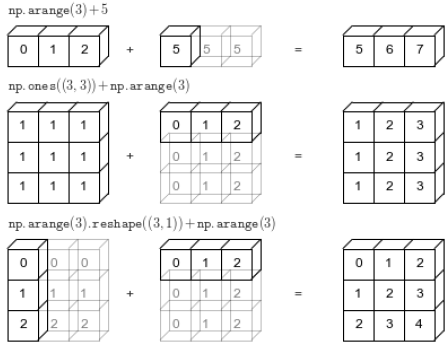
\includegraphics[width=0.5\linewidth]{imgs/lecture10/10.1 broadcasing.png}
    \caption{Broadcasting rules explained}
    \label{fig:10.1}
\end{figure}

\section{Pandas}
Pandas is an open-source library that provides high-performance, easy-to-use data structures and analysis tools. Its primary objects, \textit{Series and DataFrames}, are built on top of NumPy arrays to provide both the flexibility needed for data wrangling (like handling labeled data) and the efficiency of numerical arrays. 

\subsection{Series}
A Series is defined as a one-dimensional array of indexed data. While a NumPy array defines an implicit integer index, a Pandas Series allows for an explicitly defined index. A Series can also be thought of as a specialized type of dictionary where keys are the indices and values are the data points. \par
Examples: \par
--> data = pd.Series ([a, b, c, d], index=[1, 2, 5, 7])\par
--> data[5] returns \textit{c}

\subsection{DataFrame}
While a Series is 1D, a DataFrame is a two-dimensional array with flexible row indices and flexible column names. It can be viewed as a sequence of aligned Series objects that share the same index.

\subsection{Indexing and Selection}
Pandas can sometimes be ambiguous when using integer indices \par
--> Is data[5] refers to the explicit label or the implicit fifth position?\par
To solve this, the library provided specific indexer attributes:
\begin{itemize}[noitemsep]
    \item \textbf{loc}: always refers to the \textbf{explicit} index (the user-defined label)
    \item \textbf{iloc}: always refers to the \textbf{implicit} index (the Python-style positional index starting from 0)
    \item \textbf{ix}: a hybrid of the two, though less commonly used in the modern versions.
\end{itemize}
Examples: \par
--> data = pd.Series ([a, b, c, d], index=[1, 2, 5, 7])\par
--> data.loc[1] returns \textit{a}\par
--> data.iloc[1] returns \textit{b} \par
--> data.loc [1:2] returns {[1, a], [2, b]} \par
--> data.iloc[1, 2] returns {[2, b], [5, c]} \par
One can access the column name in a dictionary-style (--> data['population']) or in an attribute-style (--> data.population). However, the assignment works only for a dictionary-style.

\subsubsection{Indexing conventions for DataFrame}
While indexing refers to columns, slicing refers to rows. Also direct masking operations are interpreted row-wise rather than column-wise.\par
--> data[data.density > 100] returns rows of the dataframe that satisfies the condition\par
Ufuncs preserve index and column labels in the output, and for binary operations like addition and multiplication, Pandas automatically align indices.

\subsection{Handling missing data}
Pandas is particularly robust at managing "junk" or missing data. It uses \textit{None} for generic object data and \textit{NaN} for numerical values. It can automatically convert between these types when appropriate (if inserting None into an integer array will convert the array to floating-point and use NaN). \par
It offers built-in methods to work on missing data, either to fill in, to remove, or to replace. For example, \textit{dropna()}, which can remove missing values from a Series or entire rows/columns from a DataFrame.

\section{Data visualization tools in Python}
Python offers a vast and interconnected landscape of visualization libraries. At the heart is Matplotlib, which serves as the foundation for many other popular tools like Seaborn and the built-in plotting functions in Pandas. Other libraries include JavaScript-based tools like Plotly and Bokeh, and OpenGL-based tools for high-performance rendering. 

\subsubsection{Matplotlib}
This library is heavily inspired by Matlab, making it very easy for researchers moving from that environment to adapt. 

\begin{itemize}[noitemsep]
    \item \textbf{Pros}: It is extremely flexible and supports many different rendering backends
    \item \textbf{Cons}: The API is imperative (you need to tell it exactly how to draw every piece), the default style is considered poor, and it lacks interactivity; it can be slow when handling very large datasets or complex designs
\end{itemize}

\subsubsection{Matplotlib inspired tools}
\begin{itemize}[noitemsep]
    \item \textbf{Pandas}: Its goal is to provide a simple way to visualize a DataFrame directly, often including more complex graphs with less code than raw Matplotlib
    \item \textbf{Seaborn}: This library is specifically targeted toward statistical data visualization. It provides much aesthetically pleasing default "nice style" and simplifies the creation of complex plots, such as joint plots that combine scatter plots with histograms or kernel density estimates.
\end{itemize}

\subsubsection{Plotly}
It is a modern alternative to the Matplotlib family, built on JavaScript. It provided high interactivity, allowing users to zoom, hover for data, and toggle categories. While it uses JavaScript for the rendering, a version called Dahs is available that allows Python users to build interactive dashboards without needing to write any JavaScript code.

\subsubsection{Imperative vs Declarative}
Imperative means that you have to manually specify the graphs and the related details.\par
Declarative means that you have to specify what should be done with the data, and the framework decides the details.